%%%%%%%%%%%%%%%%%%%%%%%%%%%%%%%%%%%%%%%%%
% Beamer Presentation
% LaTeX Template
% Version 1.0 (10/11/12)
%
% This template has been downloaded from:
% http://www.LaTeXTemplates.com
%
% License:
% CC BY-NC-SA 3.0 (http://creativecommons.org/licenses/by-nc-sa/3.0/)
%
%%%%%%%%%%%%%%%%%%%%%%%%%%%%%%%%%%%%%%%%%

%----------------------------------------------------------------------------------------
%	PACKAGES AND THEMES
%----------------------------------------------------------------------------------------

\documentclass{beamer}

\mode<presentation> {

% The Beamer class comes with a number of default slide themes
% which change the colors and layouts of slides. Below this is a list
% of all the themes, uncomment each in turn to see what they look like.

%\usetheme{default}
%\usetheme{AnnArbor}
%\usetheme{Antibes}
%\usetheme{Bergen}
%\usetheme{Berkeley}
%\usetheme{Berlin}
%\usetheme{Boadilla}
%\usetheme{CambridgeUS}
%\usetheme{Copenhagen}
%\usetheme{Darmstadt}
%\usetheme{Dresden}
%\usetheme{Frankfurt}
%\usetheme{Goettingen}
%\usetheme{Hannover}
%\usetheme{Ilmenau}
%\usetheme{JuanLesPins}
%\usetheme{Luebeck}
%\usetheme{Madrid}
%\usetheme{Malmoe}
%\usetheme{Marburg}
%\usetheme{Montpellier}
%\usetheme{PaloAlto}
%\usetheme{Pittsburgh}
%\usetheme{Rochester}
%\usetheme{Singapore}
%\usetheme{Szeged}
\usetheme{Warsaw}

% As well as themes, the Beamer class has a number of color themes
% for any slide theme. Uncomment each of these in turn to see how it
% changes the colors of your current slide theme.

%\usecolortheme{albatross}
%\usecolortheme{beaver}
%\usecolortheme{beetle}
%\usecolortheme{crane}
%\usecolortheme{dolphin}
%\usecolortheme{dove}
%\usecolortheme{fly}
%\usecolortheme{lily}
%\usecolortheme{orchid}
%\usecolortheme{rose}
%\usecolortheme{seagull}
%\usecolortheme{seahorse}
%\usecolortheme{whale}
%\usecolortheme{wolverine}

%\setbeamertemplate{footline} % To remove the footer line in all slides uncomment this line
%\setbeamertemplate{footline}[page number] % To replace the footer line in all slides with a simple slide count uncomment this line

%\setbeamertemplate{navigation symbols}{} % To remove the navigation symbols from the bottom of all slides uncomment this line
}

\usepackage{graphicx} % Allows including images
\usepackage{booktabs} % Allows the use of \toprule, \midrule and \bottomrule in tables
\usepackage{algorithm2e}
\usepackage{algorithmic}
\renewcommand{\algorithmicrequire}{\textbf{Input:}}
\renewcommand{\algorithmicensure}{\textbf{Output:}}

%----------------------------------------------------------------------------------------
%	TITLE PAGE
%----------------------------------------------------------------------------------------

\title[Hash Tables]{Hash Tables} % The short title appears at the bottom of every slide, the full title is only on the title page

\author{Saurabh Mathur } % Your name
\institute[VIT U] % Your institution as it will appear on the bottom of every slide, may be shorthand to save space
{
VIT University \\ % Your institution for the title page
\medskip
\textit{14BIT0180} % Your email address
}
%\date{\today} % Date, can be changed to a custom date

\begin{document}

\begin{frame}
\titlepage % Print the title page as the first slide
\end{frame}

\begin{frame}
\frametitle{Overview} % Table of contents slide, comment this block out to remove it
\tableofcontents % Throughout your presentation, if you choose to use \section{} and \subsection{} commands, these will automatically be printed on this slide as an overview of your presentation
\end{frame}

%----------------------------------------------------------------------------------------
%	PRESENTATION SLIDES
%----------------------------------------------------------------------------------------

%------------------------------------------------
\section{Why use Hashing} % Sections can be created in order to organize your presentation into discrete blocks, all sections and subsections are automatically printed in the table of contents as an overview of the talk
%------------------------------------------------

\subsection{Word Count} % A subsection can be created just before a set of slides with a common theme to further break down your presentation into chunks

\begin{frame}
\frametitle{Word Count}
Read a text file, count the number of times each word appears, and print and how many times each word appears.\\\medskip
    \textbf{Input:} A sequence of $n$ words \\
    \textbf{Output:} A list of $(word, frequency)$ pairs


\end{frame}

%------------------------------------------------
\subsection{Sets} % A subsection can be created just before a set of slides with a common theme to further break down your presentation into chunks

\begin{frame}
\frametitle{Set}
Read a text file and, print each unique word.\\\medskip
    \textbf{Input:} A sequence of $n$ words \\
    \textbf{Output:} A list of $k$ unique words ($k < n$)


\end{frame}



%------------------------------------------------
\subsection{Unique data representation} % A subsection can be created just before a set of slides with a common theme to further break down your presentation into chunks

\begin{frame}
\frametitle{Unique data representation}
Read a sequence of text files and, print a string uniquely identifying each file.\\\medskip
    \textbf{Input:} A sequence of $n$ text files \\
    \textbf{Output:} A list of $n$ unique strings corresponding to each file.


\end{frame}



\section{What is a Hash Table}
\subsection{Definition}
\begin{frame}
\frametitle{Definition}
\begin{columns}[c] % The "c" option specifies centered vertical alignment while the "t" option is used for top vertical alignment

\column{.45\textwidth} % Left column and width

A \textbf{Hash Table} is a data structure used to implement the associative array ADT, a structure that can map keys to values.
\column{.5\textwidth} % Right column and width


\begin{figure}
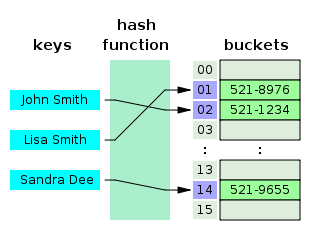
\includegraphics[width=0.8\linewidth]{hash.png}
\end{figure}


\end{columns}
\end{frame}

\subsection{Structure}
\begin{frame}
\frametitle{Structure}
A hash table consists of -
\begin{itemize}
  \item A Hash Function
  \item An array
\end{itemize}
\end{frame}

\begin{frame}
\frametitle{Hash Function}
A hash function is a function that almost uniquely maps any value (called a key) to an index in the array.
The key may be an integer, a string, a structure etc.\\
Eg. SHA-0, SHA-1, SHA-2, MD4, MD5
\end{frame}

\begin{frame}[fragile]
\frametitle{Operations}
\begin{verbatim}
  void put(Key key, Value val)
  Value get(Key key)
  void remove(Key key)
\end{verbatim}
\end{frame}

\begin{frame}
\frametitle{Collision Resolution}
\begin{itemize}
  \item Probing
  \begin{itemize}
    \item Linear
    \item Quadratic
  \end{itemize}
  \item Chaining
\end{itemize}
\end{frame}

\begin{frame}
\frametitle{Probing}
\begin{figure}
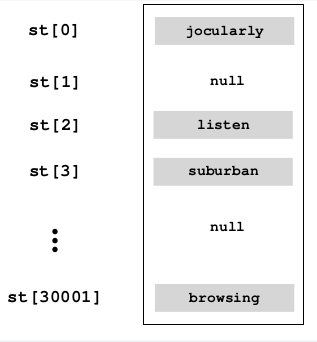
\includegraphics[width=0.4\linewidth]{probing.png}
\end{figure}
\end{frame}
\begin{frame}
\frametitle{Chaining}
\begin{figure}
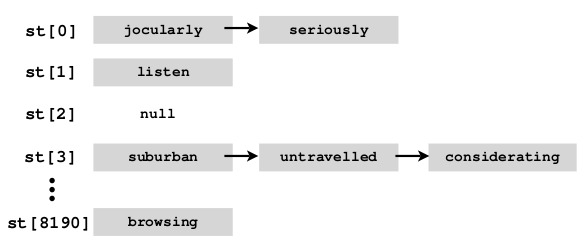
\includegraphics[width=0.8\linewidth]{chain.png}
\end{figure}
\end{frame}




\section{Anaylsis}
\subsection{Trade-offs}
\begin{frame}
\frametitle{Trade-offs}
\begin{itemize}
  \item Memory sacrificed for speed and random access.
  \item No sequential/ordered access.
\end{itemize}
\end{frame}





%------------------------------------------------
  \subsection{Asymptotic Analysis}
\begin{frame}
\frametitle{Asymptotic Analysis}
For an ideal hash, insertion, deletion and look-up are all constant time i.e. O(1)
\begin{figure}
\includegraphics[width=0.8\linewidth]{list.png}
\end{figure}


\end{frame}



\begin{frame}
\Huge{\centerline{The End}}
\end{frame}

%----------------------------------------------------------------------------------------

\end{document}
